\setlength\abovedisplayskip{2.5pt}

For relevant nuclear forensics predictions, both classification and regression
algorithms must be used.  For example, one may want to predict the reactor type
label given some measurement-based features of \gls{SNF} of an unknown source.
This would require a classification algorithm. Or perhaps the input fuel
composition is relevant to an investigation on weapons intent, so a regression
algorithm would be used. 

There are three algorithms presented in this section: \textit{k}-nearest
neighbors, decision trees, and \gls{MLL} calculations. They were chosen based
on their simplicity; this work has yet to be benchmarked using simple
algorithms so a more complex treatment of the training sets in this work would
be premature. Additionally, in part because of their simplicity, they are all
"white box" methods.  This is unique in the \gls{ML} universe, since most
algorithms create a black box model that is unable to be analyzed by a human.
The  decision trees method provides an output model that can be used to discern
behavior and understand predictions, and \textit{k}-nearest neighbors and
\gls{MLL} calculations do not create a model at all. Individual predictions can
still be analyzed, however, since the procedures are so simple. 

\subsubsection{Nearest Neighbor Methods}

Nearest neighbors classification and regression are unique algorithms in
that thay are instance-based; they do not actually generalize, but instead
track the observations in the training set.  The main metric for this algorithm
is distance (or dissimilarity) between the test sample and the closest training
sample(s) in the vicinity.  During prediction, the algorithm will calculate a
value based on the instance that is closest to the current test sample. Thus,
there is not any learning, but instead a direct comparison between an unknown
sample and the space that the training set populates. The predictions from
nearest neighbors can be quite accurate, but are highly unstable to
peturbations \cite{elements_stats}.

The process of prediction with \textit{k}-nearest neighbors is as follows.
First, the distances between the test sample and each of the training set
instances are calculated.  Most commonly the Euclidian distance is used, but
this walkthrough uses the Manhattan distance:
\begin{equation}
  d_{i} = \sum_{j=1}^{N_{feats}} |x_{j,train} - x_{j,test}|
  \label{eq:l1}
\end{equation}
where $i$ is each training set instance, and $j$ refers to each feature in the
training set.  The lowest \textit{k} $d_{i}$ are chosen. For \textit{k}-nearest
neighbors regression, the value, $y$ is predicted using the following equation.
\begin{equation}
  y(\boldsymbol{x}) = \frac{1}{k} \sum_{i=1}^{k} w_i \cdot y_i
  \label{eq:knn}
\end{equation}
where $w_{i}$ is either uniform and takes on a value of $1$ or is
distance-based and takes on a value of $1/d_{i}$ and $\boldsymbol{x}$ is the
full set of features. The regression equation averages the closest \textit{k}
neighbors for an estimate of the unknown sample.  In \textit{k}-nearest
neighbors classification, the class label $y$ is predicted using the mode of
the nearest neighbors selected using the \textit{k} smallest $d_i$, or when
$w_i$ is $1/d{i}$ the weighted mode is used to choose the predicted label.

\begin{figure}[!htb]
  \centering
  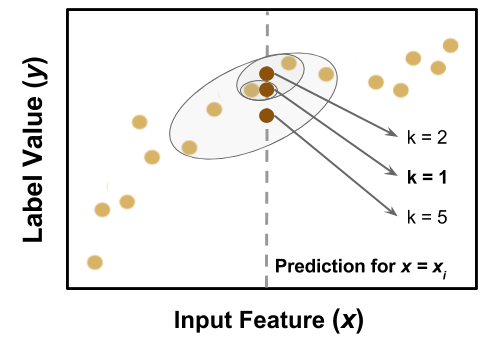
\includegraphics[width=0.8\linewidth]{./chapters/litrev/nn-fig.png}
  \caption{Schematic of \textit{k}-nearest neighbors regression, showing how 
           changing \textit{k} alters the predicted label value $y$.}
  \label{fig:nn}
\end{figure}

Figure \ref{fig:nn} provides a pictoral explanation of Equation \ref{eq:knn}
for a prediction where there is one feature. In this figure, there is a test
sample with a feature, valued at $x_i$, indicated with the grey dotted line.
The three circles represent the neighborhood given by the value of \textit{k},
and the darker dots on the line represent the reported prediction $y$ for each
choice of \textit{k}.  In this illustration, $k=1$ or $k=2$ provide a more
accurate prediction according to a visual inspection of the trend, but higher
values of $k$ can be useful, and will be discussed in Section
\ref{sec:complexity}.

\subsubsection{Decision Trees}

Decision trees are a common choice because they are simple to implement and
provide an interpretable model. However, the predictions from decision trees,
similar to \textit{k}-nearest neighbors, are unstable to peturbations.  What
follows is a highly simplified explanation of the Classification and Regression
Trees algorithm for growing decision trees, showing only the equations for
splitting criteria.  A more complete treatment can be found in Reference
\cite{elements_stats} or in the User Guide in Reference \cite{scikit}.

At their core, decision trees algorithms split the feature space into different
regions.  Decision trees are constructed by iteratively finding places in the
feature space at which to split the data to best predict a label. Some measure
of information gain (more accurately the opposite, impurity, denoted here as
$H$) is used to select a splitting criterion at each split, which maximizes
differentiation between average label values in regression or groups similar
labels together in classification.  This process continues until some
externally set stopping requirement is met, or no information gain can be made
by continuing to create splits. 

Each split creates two new nodes on the tree, where the node has to find a new
splitting criterion. In the math that follows, there are nodes given by $m$,
and a number of samples in each node given by $N_{\text{samples}, m}$. The
individual node samples are given by $i$. The impurity at the node is denoted
as $H(m)$. In classification, the node impurity can be measured by the Gini
index, where $p_{m, k}$ is the proportion of class $k$ observations at the
node:
\begin{equation}
  \begin{aligned}
    p_{m, k} &= \frac{1}{N_{\text{samples}, m}} \sum_{i=1}^{N_{\text{samples}, m}}
              I(y = k)
    \\
    H(m) &= \sum_k p_{m, k} (1 - p_{m, k})
  \end{aligned}
\end{equation}
And in regression, the node impurity $H(m)$ can be measured by the mean squared
error, where $\bar{y}_m$ is the average value of the samples in the node.
\begin{equation}
  \begin{aligned}
    \bar{y}_m &= \frac{1}{N_{\text{samples}, m}} \sum_{i=1}^{N_{\text{samples}, m}} 
                 y_{i, m}
    \\
    H(m) &= \frac{1}{N_{\text{samples}, m}} \sum_{i=1}^{N_{\text{samples}, m}}
              (y_i - \bar{y}_{i, m})^2
  \end{aligned}
\end{equation}
The splitting criterion with the lowest impurity is the one that is chosen to
make the split.  This will partition the feature space and the splitting
process will continue until a pre-defined tree size or number of samples per
node. Without a pre-defined stopping point the tree will grow until there is
one sample per node. This process can be understood more intuitively by
stuyding Figure \ref{fig:dtr}. Note that this tree was created using a maximum
tree depth of $2$ for visualization purposes in order to explain the process,
so is not indicative of a real decision tree.

\begin{figure}[!htb]
  \centering
  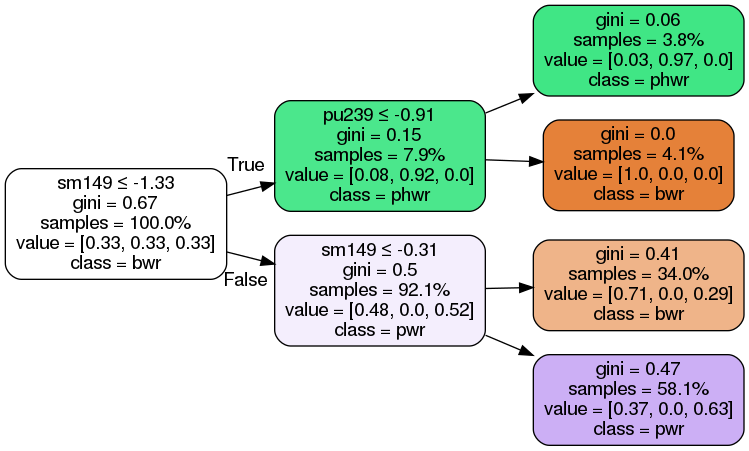
\includegraphics[width=\linewidth]{./chapters/litrev/dtree.png}
  \caption{Example of a decision tree process, where maximum tree depth was 
           limited to 2 for vizualization purposes.}
  \label{fig:dtr}
\end{figure}

In Figure \ref{fig:dtr}, the first split is determined to occur at the feature
Sm149 on whether the nuclide measurement is above a value of $-1.33$. Note that
this value is negative because of the scaling process the training set is put
through, described in Section \ref{sec:statmodel1}.\todo{check this later} The
majority class at this node is \gls{BWR} which is expected since the training
set is 72\% \gls{BWR}.  The values list indicates the fraction of each class in
the node, which is alphabetically ordered \texttt{[BWR, PHWR, PWR]}. It is even
among the three because the class weights were told to be balanced.  This
splitting criterion provides a Gini impurity score of 0.67, which represents
the minimum Gini impurity of all the candidate splits, but also indicates there
are multiple classes represented in this node (again, expected).  It would be 0
if there were only one class in the node.  In the visualization, the shading of
the colors in the tree are bolder for there being a higher fraction of a single
class.

\subsubsection{Maximum Log-Likelihood Calculations}

The \gls{MLL} calulations approach applied here is based on a method developed
to do similar work \cite{mll_method, mll_validate, mll_sensitivity}.  That work
involved matching nuclear material samples based on some select measurements to
entries in a database of containing those measurements.\todo{keep vague or no?}
Each database entry also has a similar list of labels to the labels being
predicted in this work: reactor type, burnup, and time since irradiation.

Interestingly, the \gls{MLL} calculations method works like \textit{k}-nearest
neighbors, where there is no model but a prediction according to the closest
match database entry.  There is one detail that differs, however. Whereas
\textit{k}-nearest neighbors minimizes distance/dissimilarity, this approach
instead maximizes similarity via a likelihood function. An "unknown" test
sample is compared against the training set using the likelihood calculation
between that sample and the training set entries.  The higher the likelihood,
the higher the probability that the database entry represents the sample. The
likelihood is in Equation \ref{eq:like}, whereas the log-likelihood is used
more often in practice, shown in Equation \ref{eq:loglike}.
\begin{equation}
  L(M|x_{test}) = \prod_i \frac{1}{\sigma_{i,train} \sqrt{2\pi}} \exp{\frac{-(x_{i,test} - x_{i,train})^2}{2 \sigma_{i,train}^2}}
  \label{eq:like}
\end{equation}
\begin{equation}
  ln(L(M|x_{test})) = \sum_i ln(\frac{1}{\sigma_{i,train} \sqrt{2\pi}}) - \frac{(x_{i,test} - x_{i,train})^2}{2 \sigma_{i,train}^2}
  \label{eq:loglike}
\end{equation}
The likelihood is a measure of the probability that a model $M$ produced the
measurements seen in the test sample, given by $L(M|x_{test})$.  In both
Equations \ref{eq:like} and \ref{eq:loglike}, $x$ refers to the set of
features, and $x_{i, test}$ and $x_{i,train}$ are the individual features for the
test sample and the training set entries, respectively. The uncertainty of the
measurement associated with each feature is represented by $\sigma_{i,train}$.

